\documentclass[we,final,11pt,oneside,openany]{uantwerpenbamathesis}
% \documentclass[we,a4paper,11pt,twoside,openright]{uantwerpenbamathesis}

\usepackage[english]{babel}

%% this is just for some dummy text, please remove in your copy
\usepackage{kantlipsum}
\usepackage{natbib}
\usepackage[linesnumbered,ruled,vlined]{algorithm2e}
\usepackage{listings}
\usepackage{xcolor}
\usepackage{amssymb}
\newcommand{\algorithmfootnote}[1]{\leavevmode\rlap{\footnotesize #1}\par}
\usepackage{todonotes}
\usepackage{float}

%% this package allows to generate a PDF with clickable links
\usepackage[backref,hyperindex=true,pagebackref=true]{hyperref}

\usepackage{cleveref}
%% as an example - loading some fonts, feel free to change
\usepackage{mathptmx}
\iftutex
%% Just an example of font-scheme: this is in no way a recommended font
%% scheme!
\usepackage{fontspec}
\setmainfont
[UprightFont = *,
 BoldFont = *b,
 ItalicFont = *i,
 BoldItalicFont = *z,
]
{calibri}
\usepackage{sansmathaccent}
\fi

\lstdefinestyle{bashstyle}{
  language=bash,
  basicstyle=\ttfamily\small,
  backgroundcolor=\color{gray!10},
  frame=single,
  rulecolor=\color{gray!60},
  frameround=tttt,
  keywordstyle=\color{blue},
  commentstyle=\color{green!60!black}\itshape,
  stringstyle=\color{orange},
  showstringspaces=false,
  breaklines=true,
  columns=fullflexible,
  captionpos=b,
  keywords={\$}
}

\bamadegree{we-en-ma-em}

\title{Provide a title}

\author{Inte Vleminckx}
\supervisor{prof. dr. H. Vangheluwe}{UAntwerpen}
\supervisor{R. Mittal, Doctoral Fellow}{UAntwerpen}

\academicyear{2024 - 2025}

%% you can specify a company logo
%%\companylogo{\includegraphics[width=4.5cm,height=2.5cm,keepaspectratio]{companylogo.jpg}}

\begin{document}

%% creates the title page, remove if you don't want any
\maketitle

%% causes the first pages to be roman numbered
\frontmatter

%% sets the table of contents (automatically for you)
\tableofcontents

%% changes the numbering system to arabic and restart from 1
\mainmatter

% %%%%%%%%%%%%%%%%%%%%%%%%%%%%%%%%%%%%%%%%%%%%%%%%%%%%%%%%%%% %
% %%%%%%%%%%%%%%%%%%%%%%%%%%%%%%%%%%%%%%%%%%%%%%%%%%%%%%%%%%% %
% %%%%%%%%%%%%%%%%%%%%%%%%%%%%%%%%%%%%%%%%%%%%%%%%%%%%%%%%%%% %
\chapter{Introduction}
\label{ch:introduction}

The development of products in the heating, ventilation, and air conditioning (HVAC) industry presents significant challenges in testing and validation.
Building physical prototypes for every design iteration is often costly and time-consuming.
A promising alternative is to model the most expensive or complex components in a virtual environment, enabling early testing without full-scale prototypes.
This approach allows the evaluation of critical subsystems, particularly the control software that regulates HVAC systems.

In this study, we investigate how to test the control loop of a heating and ventilation system by modeling all physical elements—such as the valve, the actuator controlling the valve, the flow sensor, the pipe network, and the pressure pump that generates the fluid flow.
The control loop, which determines the actuator setpoint based on the flow sensor measurements, will interact with the virtual model using co-simulation techniques.
To assess the feasibility and performance of this approach, we compare two testing strategies: Software-in-the-Loop (SiL), and Hardware-in-the-Loop (HiL).
In SiL testing, the model interacts with a compiled version of the control loop running on a separate system, with all connections established virtually.
In HiL testing, the model runs on one system while the control loop is executed on the actual embedded hardware used in the real setup, with physical connections between the two.

Our methodology proceeds in stages.
First, we develop a simple flow circuit in Modelica to demonstrate basic co-simulation capabilities.
Using this model, we investigate how to integrate it with SiL and HiL environments.
Once this foundation is established, we expand the Modelica component library with more detailed and realistic system elements.
Finally, we construct an advanced flow circuit model and benchmark SiL results against HiL results to evaluate performance differences and validate the modeling approach.

\todo{Inte: add what can be expected in each upcomming section in one sentece.}


% %%%%%%%%%%%%%%%%%%%%%%%%%%%%%%%%%%%%%%%%%%%%%%%%%%%%%%%%%%% %
% %%%%%%%%%%%%%%%%%%%%%%%%%%%%%%%%%%%%%%%%%%%%%%%%%%%%%%%%%%% %
% %%%%%%%%%%%%%%%%%%%%%%%%%%%%%%%%%%%%%%%%%%%%%%%%%%%%%%%%%%% %
\chapter{Proposed Approach}
\label{ch:proposed-approach}

\section{The First Steps}
\label{sec:the-first-steps}

To address the problem at hand, we must first establish a clear understanding of the overall problem statement.
As outlined in the introduction, our goal is to test the control loop of a heating and ventilation system by modeling all physical elements and allowing the control loop to interact with this model.
To achieve this, we need to define, as simply as possible, what the model requires as input from the control loop and what the control loop requires as input from the model, without yet considering detailed configuration parameters of the individual physical components.
With this understanding in place, we can represent the interaction between the control loop and the model using the following diagram:

\begin{figure}[h!]
    \centering
    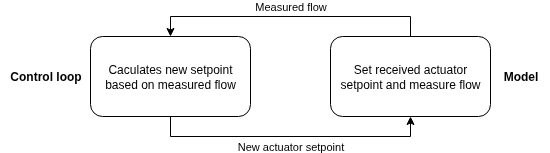
\includegraphics[width=0.6\linewidth]{Images/generated/simple-representation}
    \caption{Simple represention of interaction between control loop and model}
    \label{fig:simple-representation}
\end{figure}

Next, we provide a more detailed explanation of the process illustrated in \autoref{fig:simple-representation}.
In this setup, the control loop receives a target flow setpoint.
Although the source of this setpoint is not relevant to our study, it defines the desired flow rate in the circuit.
To achieve this flow rate, the control loop calculates an actuator setpoint, which adjusts the valve opening to provide the required flow.
In order to perform this calculation, the control loop must receive feedback from the model in the form of the measured flow in the circuit.
By comparing the measured flow to the target flow, the control loop can determine the necessary actuator setpoint and adjust the valve position accordingly.

With this simplified setup, we can construct a Modelica model that accepts one real-valued input and produces one real-valued output—the actuator setpoint and the measured flow, respectively.
For testing purposes, we can initially provide fixed output values from the model to the control loop to observe how the actuator setpoint evolves over time.
To enable full co-simulation, we must also determine how to establish interaction between the Modelica model and the control loop.
The workflow for this process is as follows:
\begin{enumerate}
    \item Develop a simple Modelica model.
    \item Investigate how the compiled control loop can be accessed and controlled using Python.
    \item Integrate the Modelica model into the Python code so that the control loop can exchange data with the model in real time.
\end{enumerate}

\subsection{A Simple Modelica Model}
\label{subsec:a-simple-modelica-model}

A very simple Modelica model can be represented as shown in \autoref{fig:simple-modelica-model}.
\begin{figure}[h!]
    \centering
    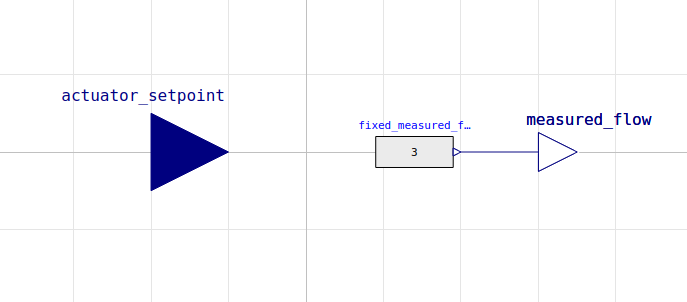
\includegraphics[width=0.6\linewidth]{Images/modelica/simple-representation}
    \caption{A simplified model representatino}
    \label{fig:simple-modelica-model}
\end{figure}

This model accepts an actuator setpoint as input and produces a measured flow as output, which is currently fixed at a value of 3 for testing purposes.

\subsection{Interaction With The Control Loop}
\label{subsec:interaction-with-the-control-loop}

The first step in enabling interaction with the control loop is to compile the common platform—containing the control loop—into an executable.
This common platform is implemented in C and is compiled using CMake.
Due to privacy regulations of the company related to this study, the source code of the common platform cannot be shared.

Once the executable is available, the next step is to establish a method for interacting with the common platform.
There are two primary communication interfaces used by the platform:

\begin{enumerate}
    \item A Flow Sensor Board (FSB), which emulates the behavior of a real flow sensor using a UART connection.
    \item A Modbus interface, which allows reading registers from the embedded control board using a TCP connection.
\end{enumerate}

In the case of Software-in-the-Loop (SiL) testing, the common platform is executed locally.
A mock Modbus connection is created to replicate the behavior of a physical Modbus link to an embedded board.
To keep the discussion focused, we first consider only the SiL setup.
A schematic representation of this communication is shown in \autoref{fig:common-platform-communication}.

\begin{figure}[h!]
    \centering
    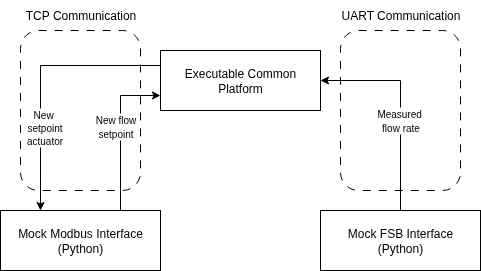
\includegraphics[width=0.6\linewidth]{Images/generated/common-platform-communication}
    \caption{Overview communication with common platform}
    \label{fig:common-platform-communication}
\end{figure}

To enable this interaction, we must first create virtual serial ports that allow communication with the common platform.
This can be achieved using the following commands:

\begin{lstlisting}[style=bashstyle, caption={Creating virtual ports for communication}]
$ sudo socat -d -d pty,link=/dev/ttyV1,raw,echo=0 pty,link=/dev/ttyV2,raw,echo=0
$ sudo chmod 777 /dev/ttyV1 && sudo chmod 777 /dev/ttyV2 && \
sudo socat -d -d -u OPEN:/dev/ttyV1,raw tcp:localhost:8888,reuseaddr
\end{lstlisting}

This configuration uses socat to create a pair of virtual serial ports and forward data through a TCP socket.
First, it establishes two pseudo-terminal devices—/dev/ttyV1 and /dev/ttyV2—which function as the two ends of a virtual null-modem cable: any data written to one port immediately appears on the other.
Next, their permissions are updated to allow unrestricted access, and a second socat process forwards all data received on /dev/ttyV1 to a TCP connection on port 8888.

The last part is to those ports using python, such that we can interact with the common platform using python code.
\todo{Go futher from here, talk about how we connect to the ports using the python Uart and TCP code}


\subsection{Complete Intergration}
\label{subsec:complete-integration}

% %%%%%%%%%%%%%%%%%%%%%%%%%%%%%%%%%%%%%%%%%%%%%%%%%%%%%%%%%%% %
% %%%%%%%%%%%%%%%%%%%%%%%%%%%%%%%%%%%%%%%%%%%%%%%%%%%%%%%%%%% %
% %%%%%%%%%%%%%%%%%%%%%%%%%%%%%%%%%%%%%%%%%%%%%%%%%%%%%%%%%%% %
\chapter{Modelica Library Overview}
\label{ch:modelica-library-overview}


% %%%%%%%%%%%%%%%%%%%%%%%%%%%%%%%%%%%%%%%%%%%%%%%%%%%%%%%%%%% %
% %%%%%%%%%%%%%%%%%%%%%%%%%%%%%%%%%%%%%%%%%%%%%%%%%%%%%%%%%%% %
% %%%%%%%%%%%%%%%%%%%%%%%%%%%%%%%%%%%%%%%%%%%%%%%%%%%%%%%%%%% %
\chapter{Results}
\label{ch:results}

% %%%%%%%%%%%%%%%%%%%%%%%%%%%%%%%%%%%%%%%%%%%%%%%%%%%%%%%%%%% %
% %%%%%%%%%%%%%%%%%%%%%%%%%%%%%%%%%%%%%%%%%%%%%%%%%%%%%%%%%%% %
% %%%%%%%%%%%%%%%%%%%%%%%%%%%%%%%%%%%%%%%%%%%%%%%%%%%%%%%%%%% %
\chapter{Conclussion}
\label{ch:conclussion}

% %%%%%%%%%%%%%%%%%%%%%%%%%%%%%%%%%%%%%%%%%%%%%%%%%%%%%%%%%%% %
% %%%%%%%%%%%%%%%%%%%%%%%%%%%%%%%%%%%%%%%%%%%%%%%%%%%%%%%%%%% %
% %%%%%%%%%%%%%%%%%%%%%%%%%%%%%%%%%%%%%%%%%%%%%%%%%%%%%%%%%%% %
\appendix

\bibliographystyle{plain}
\bibliography{refs}

\end{document}
